\chapter{Implicit Generative Models}
\section{Generative Adversarial Networks}
\label{sec:gan}
\begin{itemize}
	\item Generator's distribution: $p_{g}$
	\item Prior on input noise: $p_{z}(z)$
	\item Mapping to data space: $z\rightarrow x$ through $G(z;\theta_{g})$
	\item[] a differentiable multilayer perceptron with parameter $\theta_{g}$
	\item $D(x;\theta_{d})$: a differentiable multilayer perceptron with parameter $\theta_{d}$. It outputs a single scalar 
	\item $D(x)$: probability that $x$ (real) came from the data rather than $p_g$ (fake)
\end{itemize}

\begin{figure}[h]
	\begin{center}
		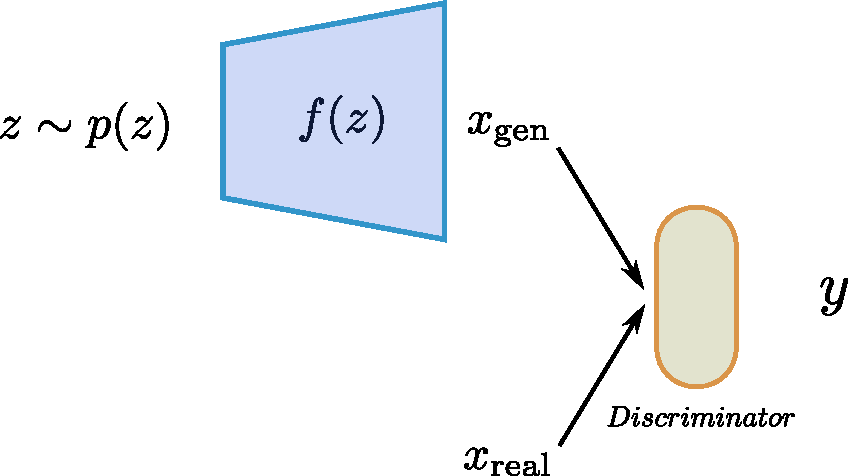
\includegraphics[scale=0.5]{./images/generative/gan/gan_model.pdf}
	\end{center}
	\caption{GAN structure}
	\label{fig:gan}
\end{figure}

\subsection{Discriminator}
The discriminator's goal is to maximize the following equation given $G$
\begin{equation*}
\mathbbm{E}_{x \sim p_{data}(x)}\log(D(x))+\mathbbm{E}_{z \sim p_{z}(z)}\log(1-D(G(z)))
\end{equation*}
The optimal discriminator given $G$ can be denoted as $D^*_{G}$. To get the optimal discriminator, define a value function
\begin{equation*}
V(G,D):= \mathbbm{E}_{x \sim p_{data}(x)}\log(D(x))+\mathbbm{E}_{z \sim p_z(z)}\log(1-D(G(z))).
\end{equation*}
Then, $D_G^* = \text{argmax}_D V(G,D)$

However, the generator $G$ wants to minimize the value function given $D=D^*_G$. 
\begin{equation*}
G^* = \text{argmin}_G V(G,D_G^*).
\end{equation*}

\begin{equation*}
\min_{G}\max_{D}V(D,G) =  \mathbbm{E}_{x\sim p_{data}(x)}[\textrm{log}D(x)]+\mathbbm{E}_{z\sim p_{z}(z)}[\textrm{log}(1-D(G(z)))]
\end{equation*}
\begin{itemize}
	\item $\min_{G} \rightarrow$ try to generate fake data that is similar to real data
	\item $\max_{D} \rightarrow$ try to assign correct label \footnotemark
\end{itemize}

At this point, we must show that this optimization problem has a unique solution $G^*$ and that this solution satisfies $p_G=p_{data}$.

\footnotetext{The above equation is trained separately at the same time, don't get confused}

One big idea from the GAN paper–, which is different from other approaches is that $G$ \textbf{need not be invertible}. Many pieces of notes online miss this fact when they try to replicate the proof and incorrectly use the change of variables formula from calculus (which would depend on $G$ being invertible). Rather, the whole proof relies on this equality:
\begin{equation*}
	\mathbbm{E}_{z \sim p_{z}(z)}\log(1-D(G(z))) = \mathbbm{E}_{x \sim p_{G}(x)}\log(1-D(x)) .
\end{equation*}

With the above equality, 
\begin{align*}
	&\mathbbm{E}_{x \sim p_{data}(x)}\log(D(x))+\mathbbm{E}_{z \sim p_z(z)}\log(1-D(G(z)))\\
	&=\int_{x} p_{data}(x)\log D(x) \, \mathrm{d}x + \int_{z} p(z)\log ( 1- D(G(z))) \, \mathrm{d}z\\ 
	&= \int_{x} p_{data}(x)\log D(x) + p_G(x) \log ( 1- D(x)) \, \mathrm{d}x
\end{align*}

Additionally, we will use the following property:
\begin{align*}
	f(y)= a \log y + b \log(1-y).
\end{align*}
To find a critical point,
$$f^\prime(y) = 0 \Rightarrow \frac{a}{y} - \frac{b}{1-y} = 0 \Rightarrow y = \frac{a}{a+b}$$
If $a+b\neq0$, do the second derivative test:
$$f^{\prime\prime}\big ( \frac{a}{a+b} \big) = - \frac{a}{(\frac{a}{a+b})^2} - \frac{b}{(1-\frac{a}{a+b})^2} < 0
$$
If $a,b\in (0,1)$, $\frac{a}{a+b}$ is a maximum.

By rewriting the equation,
\begin{align*}
V(G,D) &= \int_{x} p_{data}(x)\log D(x) + p_G(x) \log ( 1- D(x)) \, \mathrm{d}x \\
& \leq \int_x \max_y {p_{data}(x)\log y + p_G(x) \log ( 1- y)}\, \mathrm{d}x 
\end{align*}
Thus, if $D(x) = \frac{p_{data}}{p_{data}+p_G}$, then we can achieve the maximum $V(G,D)$. 

\subsection{Generator}
If we achieve the optimal $G$ (i.e., $p_G = p_{data}$), then $D$ would be completely confused and $D^*_G(x) = \frac{p_{data}}{p_{data}+p_G}=\frac{1}{2}$ (it means that $D$ cannot make a clear decision.).

The global minimum of the virtual training criterion $C(G)=\max_DV(G,D)$ is acheived if and only if $p_{G}=p_{data}$. Let's plug $D^*_G(x)$ into the criterion then, 
\begin{equation*}
	C(G) = \int_{x} p_{data}(x)\log \big (\frac{p_{data}(x)}{p_{G}(x)+p_{data}(x)} \big )  + p_G(x) \log\big ( \frac{p_{G}(x)}{p_{G}(x)+p_{data}(x)}\big ) \, \mathrm{d}x. 
\end{equation*}
To get the minimum $C(G)$, we can use the Jansen-Shannon divergence:

\begin{align*}
	D_{JS}(p_{data}||p_{G}) & = \frac{1}{2}\Bigg[D_{KL}\Big(p_{data}\Big|\Big|\frac{p_{data}+p_{G}}{2}\Big)+D_{KL}\Big(p_{G}\Big|\Big|\frac{p_{data}+p_{G}}{2}\Big)\Bigg]\\
	& = \frac{1}{2}\Bigg[\Bigg(\int_x p_{data}(x)\textrm{log}\Bigg(\frac{2p_{data}(x)}{p_{data}(x)+p_{G}(x)}\Bigg)dx\Bigg)+\Bigg(\int_x p_{G}(x)\textrm{log}\Bigg(\frac{2p_{G}(x)}{p_{data}(x)+p_{G}(x)}\Bigg)dx\Bigg)\Bigg]\\
	& = \frac{1}{2}\Bigg[\Bigg(\int_x p_{data}(x)\textrm{log}2+p_{data}(x)\textrm{log}\Bigg(\frac{p_{data}(x)}{p_{data}(x)+p_{G}(x)}\Bigg)dx\Bigg)+\\
	&\hspace{1cm}\Bigg(\int_x p_{G}(x)\textrm{log}2+p_{G}(x)\textrm{log}\Bigg(\frac{p_{G}(x)}{p_{data}(x)+p_{G}(x)}\Bigg)dx\Bigg)\Bigg]\\
	& = \frac{1}{2}\Bigg[\Bigg(\textrm{log}2+\int_x p_{data}(x)\textrm{log}\Bigg(\frac{2p_{data}(x)}{p_{data}(x)+p_{G}(x)}\Bigg)dx\Bigg)+\\
	& \hspace{1cm}\Bigg(\textrm{log}2+\int_x p_{G}(x)\textrm{log}\Bigg(\frac{2p_{G}(x)}{p_{data}(x)+p_{G}(x)}\Bigg)dx\Bigg)\Bigg]\\
	& = \frac{1}{2}(\textrm{log}4+C(G))
\end{align*}

Thus,
$$C(G) = -\textrm{log}4 + 2D_{JS}(p_{data}||p_{G})$$

Since the Jensen-Shannon divergence between two distributions is always non-negative and zero only when they are equal, we have shown that $C^* = -\textrm{log}(4)$ is the global minimum of $C(G)$ and that the only solution is $p_G=p_{data}$, i.e., the generative model perfectly replicating the data generating process.

\begin{figure}[h]
	\centering
	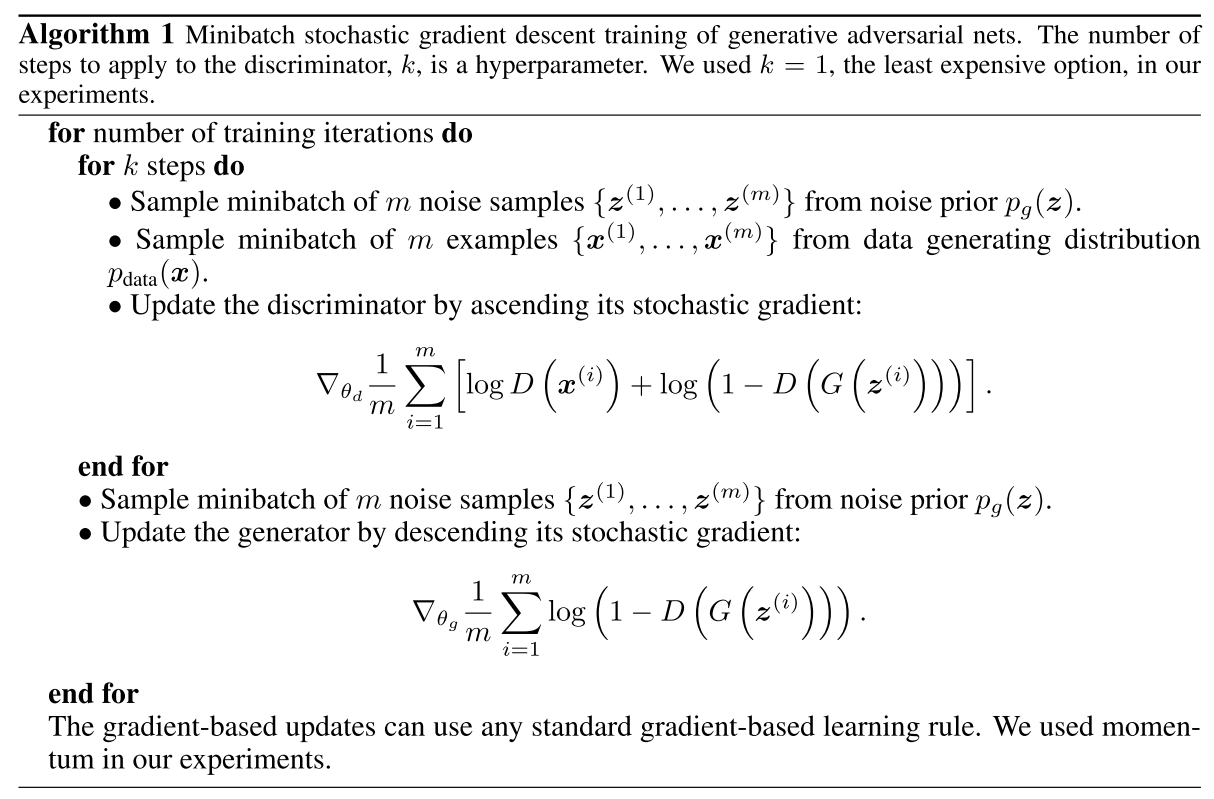
\includegraphics[scale=0.3]{./images/generative/gan/gan_algorithm.png}
	\caption{Training GAN}
	\label{fig:algorithm}
\end{figure}

\section{Some notes}
What would be the optimal discriminator that separates the two different distributions $p(x)$ and $q(x)$? It turns out that it is
$$f(x) = \frac{q(x)}{p(x)+q(x)}$$
Actually, there are many choices for classifiers e.g., KL-divergence

\begin{enumerate}
	\item What do we need to learn a classifier?
	\begin{itemize}
		\item Only samples from $p(x)$ and $q(x)$
	\end{itemize}
	\item How do we parameterize $q(x)$?
	\begin{itemize}
		\item Parametric density function (Gaussian)
		\item Define implicitly (GANs approach): define mapping from one (noise) to another (data or image)
	\end{itemize}
\end{enumerate}

The orignal GAN does not learn the data distributions. 




